\documentclass[letterpaper, 12pt]{report}
\usepackage[top = 1.8cm, left = 3cm, right = 3cm ]{geometry}
\usepackage[pdftex]{graphicx}
\usepackage[francais]{babel}
\usepackage{amsmath}
\usepackage{amsthm}
\usepackage{url}
\usepackage{tikz}
\usepackage{float}
\usepackage{listings}
\usepackage[T1]{fontenc}
\usepackage[utf8]{inputenc}
\usepackage{epigraph}
\usepackage{fancyhdr}
\usepackage{gensymb}
\usepackage{rotating}
\usepackage[french,ruled,vlined]{algorithm2e}
\usepackage{longtable}
\usepackage{newfloat}
\usepackage{enumitem}
\usepackage{amsfonts}

\DeclareFloatingEnvironment[placement={!ht},name=List]{mylist}
\theoremstyle{definition}
\newtheorem{mydef}{Definition}
\newtheorem{myprop}{Property}
\newtheorem{mylemma}{Lemma}
\newtheorem{myexample}{Example}

\newcommand{\dom}{\mathbf{dom}}
\newcommand{\att}[1]{{\mathsf{#1}}}
\newcommand{\na}{\att{Name}}
\newcommand{\cp}{\att{CP}}
\newcommand{\bd}{\att{Birthday}}
\newcommand{\yr}{\att{Year}}
\newcommand{\ta}{\att{Tax}}
\newcommand{\ic}{\att{Income}}
\newcommand{\lrformula}[1]{\left({#1}\right)}

\def\changemargin#1#2{\list{}{\rightmargin#2\leftmargin#1}\item[]}
\let\endchangemargin=\endlist 

\newcommand{\alinea}{
\hspace*{0.5cm}}

\renewcommand*\sfdefault{phv}
\renewcommand*\rmdefault{ppl}

\renewcommand\epigraphflush{flushright}
\renewcommand\epigraphsize{\normalsize}
\setlength\epigraphwidth{0.7\textwidth}

\definecolor{titlepagecolor}{RGB}{255,20,20}

\DeclareFixedFont{\titlefont}{T1}{phv}{\seriesdefault}{n}{0.375in}
  

\makeatletter
\setcounter{secnumdepth}{3} 
%\setcounter{tocdepth}{3} % makes the subsubsection appear in the table of content.
%\@addtoreset{section}{part}
%
%\renewcommand{\partname}{Partie}


% The following code is borrowed from: http://tex.stackexchange.com/a/86310/10898

\newcommand\titlepagedecoration{%
\begin{tikzpicture}[remember picture,overlay,shorten >= -10pt]

\coordinate (aux1) at ([yshift=-50pt]current page.north east);
\coordinate (aux2) at ([yshift=-380pt]current page.north east);
\coordinate (aux3) at ([xshift=-5cm]current page.north east);
\coordinate (aux4) at ([yshift=-130pt]current page.north east);
\coordinate (aux5) at ([yshift=-4cm]current page.north west);
\coordinate (aux6) at ([xshift=4cm]current page.north west);


\begin{scope}[titlepagecolor!40,line width=12pt,rounded corners=12pt]
\draw
  (aux1) -- coordinate (a)
  ++(225:5) --
  ++(-45:5.1) coordinate (b);
\draw[shorten <= -10pt]
  (aux3) --
  (a) --
  (aux1);
\draw[opacity=0.6,titlepagecolor,shorten <= -10pt]
  (b) --
  ++(225:2.2) --
  ++(-45:2.2);
\draw[opacity=0.5,titlepagecolor,shorten <= -15pt]
  (aux5) --
  (aux6);
\end{scope}
\draw[titlepagecolor,line width=8pt,rounded corners=8pt,shorten <= -10pt]
  (aux4) --
  ++(225:0.8) --
  ++(-45:0.8);

\begin{scope}[titlepagecolor!70,line width=6pt,rounded corners=8pt]
\end{scope}
\end{tikzpicture}%
}

\begin{document}
\begin{titlepage}

\noindent


\newgeometry{bottom = 2cm, top = 2.5cm}
\begin{center}

\includegraphics[scale=0.2]{umonslogo}\\
\vspace*{0.7cm}

\includegraphics[scale=0.32]{fs-logo}\\
\vspace*{2.5cm}
\titlefont Mémoire\\~\\{\LARGE  Data Repairing\\}~\\~\\{\large} \par
\end{center}
\vspace*{3.5cm}
\hfill
\begin{minipage}{0.18\linewidth}
  \begin{flushright}
   \rule{0.5pt}{75pt}
  \end{flushright}
\end{minipage}
\begin{minipage}{0.8\linewidth}
\begin{flushleft}
\textsf{\textbf{Project made by:}} Maxime Van Herzeele\\
\textsf{\textbf{Academic Year:}} 2017-2018\\
\textsf{\textbf{Dissertation director:}} Jef Wijsen\\
%\textsf{\textbf{Rapporteurs}} Pierre Hauweele \& Tom Mens\\
\textsf{\textbf{Section:}} 2$^{nd}$ Master Bloc in ComputerSciences
\end{flushleft}
\end{minipage}
\vspace*{\fill}
\begin{center}
Faculté des Sciences $\bullet$ University of Mons $\bullet$ Place du Parc 20 $\bullet$ B-7000 Mons
\end{center}
\titlepagedecoration
\end{titlepage}

\newgeometry{top = 3cm, left = 2.5cm, right = 2.5cm}

\pagestyle{fancy}
\lhead{Maxime Van Herzeele}
\rhead{MAB2 Computer Sciences}
\cfoot{\thepage}

\pagenumbering{roman} \setcounter{page}{1} 

%\section*{Remerciements} 
%\vspace*{0.8cm}
%\addcontentsline{toc}{section}{acknowledgement} 
%Todo : remerciement
%\newpage

\tableofcontents
\pagebreak
\listoffigures
\listoftables
\pagebreak

\chapter{Introduction}

\pagenumbering{arabic} \setcounter{page}{1} 

\alinea De nombreuses institutions et entreprises collectent, stockent et utilisent de nombreuses informations. Ces données peuvent être \emph{erronées} ce qui peut induire en erreur n'importe quelle personne voulant utiliser la base de données. Afin d'éviter ce problème, les données devraient respecter les contraintes d'intégrités. Ces contraintes sont des règles devant être respectées par les données, et n'importe quelle information qui ne les respectent pas est considérées comme étant erronée. Malheureusement, ces contraintes peuvent être imprécises et par conséquent elle peuvent échouée dans la différenciation entre les bonnes données et les données erronées. Pour cette raison, certaines données sont identifiées comme étant des violations de ces contraintes (données erronées) malgré qu'elles ne le devraient pas et d'un autre côté, certaines données ne sont pas identifiées comme étant des violations alors qu'elles le devraient. Ces erreurs à la fois sur les données et sur les contraintes, sont un problème pour quiconque souhaite utiliser la base de donnée.\\

Par exemple, durant mon stage en entreprise, j'ai pu travailler sur un projet associé de près à une base de données ayant ce problème semblable. Cela a eu un énorme impact sur une partie de mon projet. Le projet de réparation de ces données est prévu pour le courant de l'année 2018.\\

Le terme \emph{Data repairing} ou réparation de données signifie réparer les données mais aussi réparer les contraintes d'intégrité. Il serait naïf de penser que l'on puisse supprimer des données erronées comme on le souhaite. La perte d'information serait important parce que une telle pratique demanderait d'effacer une ligne complète de la table et ce malgré qu'il n'y ait qu'une seule erreur dans la ligne. En outre, les contraintes d'intégrité peuvent aussi ne pas être correcte ce qui veut dire que l'on pourrait supprimer une ligne ne contenant que des données correctes. Pour cette raison, nous avons besoin de techniques afin de réparer à la fois les données et les contraintes et ce sans perdre trop d'information tout en évitant d'échouer dans la détection d'erreurs dans les données.\\

Dans cette thèse de mémoire, nous allons analyser le \emph{modèle de réparation $\theta$-tolérant} comme il a été introduit dans un papier scientifique\cite{main}. Dans un premier temps nous allons introduire le concept de \emph{denial constraint}, une forme de contraintes d'intégrité qui va nous aider à définir et comprendre le concept du modèle de réparation $\theta$-tolérant. Nous allons également introduire quelques bases de données que nous utiliserons pour illustrer les différentes notions que nous allons aborder. Ensuite, nous allons présenter une implémentation du modèle $\theta$-tolérant. Et enfin, nous terminerons par une analyse des performances de l'implémentation du modèle.

\chapter{Les contraintes d'intégrité}

\alinea Dans ce chapitre, nous allons rappeler quelques notions bien connues mais nous allons également introduire de nouveaux concept. Dans un premier temps nous allons introduire quelques bases de données que nous utiliserons en tant qu'exemple pour expliquer et illustrer de nombreuses propriétes et définitions. Ces bases de données suivent le modèle relationnel qui a été introduit par E.F. Codd \cite{misc1}. Ensuite nous allons travailler sur les contraintes d'intégrités et nous allons introduire un nouveau type de contrainte appelé \emph{denial constraint}. Nous allons expliquer plusieurs caractéristiques et propriétés de ces contraintes et expliquer pourquoi nous n'utilisons pas une forme plus conventionnel de contrainte, comme par exemple les dépendances fonctionnelles.

\section{Base de données}

\alinea Dans cette section nous allons présenter des bases de données que nous allons utiliser comme exemple dans cette thèse de mémoire. Nous utiliser ces bases de données pour illustrer le modèle de réparation de données $\theta$-tolérant ainsi que d'autres notions que nous définirons.\\

La première base de données est tirée de l'article principal utilisés dans la bibliographie de cette thèse \cite{main}.

\begin{table}[H]
	\centering
	\begin{tabular}{|c|c c c c c c|}
	\hline
	    & Nom & Anniversaire & NumTel & Année & Revenu & Taxe\\
	\hline
	 t1 & Ayres & 8-8-1984 & 322-573 & 2007 & 21k & 0\\
	 t2 & Ayres & 5-1-1960 & ***-389 & 2007 & 22k & 0 \\
	 t3 & Ayres & 5-1-1960 & 564-389 & 2007 & 22k & 0 \\
	 t4 & Stanley & 13-8-1987 & 868-701 & 2007 & 23k & 3k\\
	 t5 & Stanley & 31-7-1983 & ***-198 & 2007 & 24k & 0\\
	 t6 & Stanley & 31-7-1983 & 930-198 & 2008 & 24k & 0\\
	 t7 & Dustin & 2-12-1985 & 179-924 & 2008 & 25k & 0 \\
	 t8 & Dustin & 5-9-1980 & ***-870 & 2008 & 100k & 21k \\
	 t9 & Dustin & 5-9-1980 & 824-870 & 2009 & 100k & 21k \\
	 t10 & Dustin & 9-4-1984 & 387-215 & 2009 & 150k & 40k \\
	 \hline
	\end{tabular}
	\caption{\label{tableMain} Base de données de l'article principal \cite{main}}.
\end{table}

La seconde base de données que nous allons utiliser est inspiré d'une expérience personnelle. Lors d'un stage en entreprise, j'ai pu travailler sur un projet lié à une base de donnée contenant des données erronées. Ces données ne pouvant pas être utilisé en dehors de l'entreprise, nous utiliserons une base de données reprenant l'idée générale. C'est une table appelée 'Personne' contenant différentes informations basiques sur des personnes en Belgique \footnote{Les données sont fictives} . 

\begin{itemize}
\item \textbf{NISS:} Le numéro national de la personne. Un numéro national est unique. En règle général, un NISS est formé de la manière suivante: \cite{bcss}
	\begin{itemize}
	\item Il commence avec la date de naissance de la personne dans un format YY-MM-DD. Des exceptions existe pour les étranger (c'est à dire des personne n'ayant pas la nationalité Belge) mais nous n'allons pas considérer ces cas. En effet ces cas peuvent être difficile à comprendre et ne sont aucunement intéressant pour la suite.
	\item Le nombre composé du septième, huitième et neuvième chiffres est pair pour les hommes et impair pour les femmes
	\item Le nombre composé des deux derniers chiffres est le resulat de is $n \mod 97$ avec n le nombre formé des 9 premiers chiffres
	\end{itemize}
\item \textbf{Nom:} Nom de famille de la personne.
\item \textbf{Prénom:} Prénom de la personne.
\item \textbf{Nai\_Date:} Date de naissance de la personne dans le format DD-MM-YYYY.
\item \textbf{Dec\_Date:} Date de décès de la personne dans le format DD-MM-YYYY.
\item \textbf{Etat\_Civil:} État civil courant de la personne, celui ci doit être parmi les suivants : (célibataire, décédés, marié, divorcé, décédé, veuf)
\item \textbf{Ville} : La ville où la personne vit.
\item \textbf{Code\_Post} : Le code postal de la ville.
\item \textbf{Salaire} : Le salaire perçu par la personne en une année.
\item \textbf{Taxe} : Le montant de taxe payé par la personne en une année.
\item \textbf{Enfant} : Le nombre d'enfant que la personne a à charge.
\end{itemize}

\begin{table}[H]
 \footnotesize	
	\centering
	\hspace*{-2cm}\begin{tabular}{|c|c c c c c c c c c c c|}
	\hline
	    & Niss & Nom & Prénom & Nai\_Date & Dec\_Date & Etat\_Civil & Ville & Code\_Post & Salaire & Taxe & Enfant\\
	\hline
	 t1 & 14050250845 & Dupont & Jean & 14-05-1902 & 18-05-1962 & décédé & Ath & 7822 & 25k & 4k & 2\\
	 t2 & 08042910402 & Brel & Jacques & 08-04-1929 & 09-10-1978 & décédé & Schaerbeek & 1030 & 100k & 8k & 1\\
	 t3 & 45060710204 & Merckx & Eddy & 07-06-1945 & null & décédé & Schaerbeek & 1030 & 125k & 9k & 2\\
	\hline
	 
	 \hline
	\end{tabular}
	\caption{\label{tablePerson} La table Personne}.
\end{table}


\newpage

\section{Contraintes sur les bases de données}

\alinea Les bases de données devraient n'accepter que des valeurs qui respectent certaines normes en relation avec la base de données. Ce serait un problème si on pouvait ajouter n'importe quelle valeur à chaque colonne d'une base de données. Pour eviter ce problème nous avons recours à des règles sur les bases de données. Ces règles sont appelées \emph{contraintes d'intégrité} et fonctionnent de la manière suivante: Si un tuple $t$ respecte toutes les conditions alors les données sont acceptables. Sinon $t$ n'est pas correcte et au moins une des valeurs du tuple est erronée.

Le modèle relationnel des bases de données introduit la notion de \emph{dépendance fonctionnelle}:

\begin{mydef}
Une \textbf{dépendance fonctionnelle (DF)} est une expression $X \rightarrow Y$ avec $X,Y \subseteq
sort(R)$ et où $sort(R) = \{ A_1,A_2,...,A_n\}$
\end{mydef} 

En d'autre mots, la contrainte $X \rightarrow Y$ signifie que pour une valeur spécifique de X, il n'y a au plus une valeur possible pour Y. Si la DF est respectée sur la relation R, nous pouvons dire que R satisfait la DF. Prenons quelques exemple sur la table \ref{tablePerson}:

\begin{enumerate}
\item \emph{Un NISS identifie une personne}: En d'autre mot, pour une valeur spécifique du NISS, il n'y a qu'une seule valeur possible pour tout le reste de la table. Cela peut se décrire par la DF suivante:
$ NISS \rightarrow Nom, Prénom, Nai\_Date, Dec\_Date, Etat\_Civil, Ville, Code\_Post, Salaire, Taxe, Enfant$
\item \emph{Deux personnes avec le même code postal vivent dans la même ville.} : Pour une valeur spécifique de $Code\_Post$ dans notre table il n'y a qu'une valeur possible de $Ville$. Par exemple si la valeur de $Code\_Post$ d'une personne est '7822', la seule valeur possible pour l'attribut $Ville$ est 'Ath'. La dépendance fonctionnelle dans ce cas est $Code\_Post \rightarrow Ville$.
%\item \emph{If someone died the march 18$^{th}$ 1962 , his civil status should be equal to decease.} : In this case we need a conditional functional dependency(CFD) which is typically a functional dependency with equality operator on some columns. A functional dependency should work for all records on the table, CFD can hold some conditions on collumns. $[Decease\_date = $'18-05-1962'$] \rightarrow [civil\_status = decease]$
\end{enumerate}

Si pour chaque tuple de la relation $R$, la DF $\tau$ est respectée, nous disons que la relation $R$ \emph{satisfait $\tau$}. Cela ce note $R \models \tau$. Évidement, certaines bases de données ne contiennent pas qu'une seule contrainte mais plusieurs. Il est important qu'elle soient toute respectée. Définissons cela comme ceci: 
  
\begin{mydef}
Soit un ensemble $\Sigma$ de DF sur la relation $R$. On dit que la relation $R$ satisfait $\Sigma$ noté $R \models \Sigma$ si pour chaque DF $ \tau \in \Sigma$, on a $R \models \tau$
\end{mydef}

Malheureusement les dépendances fonctionnelles sont limitées en terme de puissance. En effet, il existe de nombreuses contraintes que nous ne pouvons pas exprimer avec une DF. Par exemple, si nous souhaitons exprimer le fait que \emph{'Une personne ne peut être née avant sa propre mort'}, nous avons besoin de comparer la $Nai\_Date$ et la $Dec\_Date$ de la personne et de s'assurer que la date de décès ne soit antérieure à la date de naissance. Les dépendances fonctionnelles ne permettent pas d'utiliser des opérateurs de comparaison, il est donc nécessaire d'exprimer les contraintes d'une autre façon. Pour ce faire nous allons introduire un nouveau type de contrainte qui répondra bien à nos besoins: les \emph{denial constraints}.

\section{Les Denials constraints}

Dans cette section nous allons définir ce qu'est une denial constraint. Nous allons aussi expliquer son utilisation dans les bases de données et nous allons également lister et expliquer plusieurs propriétés que peuvent avoir ces contraintes. Commençons d'abord par définir la denial constraint

\begin{mydef}
Considérons un schéma de relation $R$ avec un ensemble $S$ fini d'\emph{attribut}. Une \emph{denial constraint (DC)} sur l'ensemble $S$ est une fonction partielle qui associe l'ensemble $S$ vers le powerset $OP$ de $\{ <,=,> \}$. Nous utiliserons la lettre grecque $\varphi$ pour représenter une DC
\end{mydef}

\begin{mydef}
 Soit $(\dom,\leq)$ un domaine totalement ordonné contenant au moins deux éléments distincts. Un \emph{tuple sur $S$} est une fonction totale de S à $\dom$. Une \emph{relation sur S} est un ensemble fini de tuples sur $S$. 
\end{mydef}

Par définition le powerset d'un ensemble $S$ noté $\mathcal{P}(S)$ est l'ensemble de tous les sous-ensemble de $S$. Cela inclut l'ensemble $S$ lui même mais aussi l'ensemble vide $\emptyset$. Par exemple le powerset de $OP$ est $\mathcal{P}(OP)$ = $\{ \emptyset, \{<\} , \{=\}, \{>\}, \{<,=\}, \{=,>\}, \{<,>\}, \{<,=,>\} \}$. Il existe différentes abréviations pour les éléments de $OP$, ceux-ci étant répertorié dans la table \ref{operatorTable}. Nous avons eu besoin d'introduire 2 nouveaux opérateur $\top$ et $\bot$, chacun étant l'abréviation pour l'ensemble $\{<,=,>\}$ et $\emptyset$ respectivement. Nous les définissons comme tel: $ \forall a,b \in \mathbf{dom}$,nous avons $d_1 \bot d_2$ est toujours faux et $d_1 \top d_2$ est toujours vrai. Nous utiliserons la lettre grecque $\phi$ ou $\theta$ pour représenter un opérateur.\\

\begin{table}
	\begin{center}
	\begin{tabular}{|c|c|c|c|c|}\hline
	Élément & Abréviation & inverse & réciproque & implication\\\hline\hline
	$\emptyset$ & $\bot$ & $\top$ & $\bot$ & $\{\bot\}$\\\hline
	$\{<\}$     & $<$ & $\geq$ & $>$ & $\{<,\leq,\neq, \top \}$\\\hline
	$\{=\}$     & $=$ & $\neq$ & $=$ & $\{=,\leq,\geq, \top \}$\\\hline
	$\{>\}$     & $>$ & $\leq$ & $<$ & $\{ >,\geq,\neq,\top \}$\\\hline 
	$\{<,=\}$   & $\leq$ & $>$ & $\geq$ & $\{\leq, \top \}$\\\hline 
	$\{<,>\}$   & $\neq$ & $=$ & $\neq$ & $\{\geq, \top \}$\\\hline
	$\{>,=\}$   & $\geq$ & $<$& $\leq$ & $\{\neq, \top \}$\\\hline 
	$\{<,=,>\}$ & $\top$ & $\bot$ & $\top$ & $\{\top \}$\\\hline
	\end{tabular}
	\end{center}
	\caption{Element de OP, le powerset of $\{ <,=,>\}$ \label{operatorTable}}
\end{table}

Expliquons maintenant la sémantique qui se cache derrière la denial constraint.

\begin{mydef}
On dit qu'une relation $I$ sur $S$ \emph{satisfait} la DC $\varphi$, noté $I \models \varphi$ si il \textbf{n'existe pas} deux tuples $s,t \in I$ tel que pour chaque attribut $A$ dans le domaine de $\varphi$, nous avons $s(A)\theta t(A)$ avec $\theta =  \varphi(A)$ 
\end{mydef}

Prenons un exemple sur la table \ref{tableMain}, nous avons $S=\{Nom,Anniversaire,NumTel,Année,Revenu,Taxe \}$ Une DC pour S est $\varphi =\{(Nom,=),(Anniversaire,=),(NumTel,\neq),(Annee,\top),(Revenu,\top) ,(Taxe,\top) \}$. Celle-ci est satisfaite par la relation $I$ si il n'existe pas deux tuples $s,t\in I$ tel que $s(Nom) = t(Nom) \wedge s(Anniversaire) = t(Anniversaire) \wedge s(NumTel) \neq t(NumTel) \wedge s(Annee) \top y(Annee) \wedge s(Revenu) \top t(Revenu) \wedge s(Taxe) \top t(Taxe)$.\\

Soit $\varphi$ une DC sur $S$ . Nous appellerons \emph{prédicat} $P$ chaque chaque couple $(A,\varphi(A))$ de $\varphi$ avec $A\in S$. Soit $pred(\varphi)$ l'ensemble des prédicats de la DC $\varphi$. Soit $I$ une relation sur $S$. Dès lors on peut dire que $\varphi$ est satisfaite si au moins un des prédicats est faux. Si un prédicat $P$ a pour opérateur $\top$ alors $P$ sera toujours vrai pour tout $t,s \in I$. Dès lors à l'avenir, nous ne noterons plus les prédicats ayant $top$ pour opéraeur par facilité syntaxique. L'exemple précédent s'écrira désormais$\varphi =\{(Nom,=),(Anniversaire,=)$. Si un prédicat a pour opérateur $\bot$, il sera toujours faux. Dès lors $I \not\models \varphi$. La DC $\varphi = \{(A_1,\top),(A_2,\top),...(A_n,\top)\} \equiv \{ \}$ n'est satisfaite par aucune relation excepté par une relation vide.\\

 Si nous prenons I comme étant la table \ref{tableMain}, nous avons $I \not\models \varphi$. En effet prenons $s=t_2$ et $t=t_3$ nous avons bien $t_2(Nom) = t_3(Nom) \wedge t_2(Anniversaire) = t_2(Anniversaire) \wedge y_2(NumTel) \neq t_3(NumTel)$. On dit que $\langle t_2,t_3 \rangle$ \emph{viole} la contrainte $\varphi$\\ 

Pour chaque opérateur dans $OP$ nous pouvons définir son inverse, sa réciproque et son implication. Les valeurs de l'inverse, la réciproque et l'implication de chaque élément de $OP$ se trouve également à la table \ref{operatorTable}.
\begin{mydef}
Soit $\phi$ un élément de $OP$

L'inverse de $\phi$ noté $\overline{\phi}$ est égal à $\{<,=,>\}\setminus \emptyset$

La réciproque de $\phi$ noté $\hat{\phi}$ s'obtient en inter-changeant < et > dans $\phi$

L'implication de $\phi$ noté $Imp(\phi)$ est un ensemble d'élément de $OP$ tel que pour n'importe quelle valeur a et b, si $a \phi_2 b$ \textbf{implique}\footnote{Tout tuple qui satisfait $a \phi_2 b$ satisfait $a \phi_1 b$} \textbf{toujours} $a \phi_1  b$ alors $\phi_2       \in Imp(\phi_1)$.
\end{mydef}

Notons que $\forall \phi_1,\phi_2$, si $\phi_2 \in Imp(\phi_1)$ alors $\phi$ est un sous ensemble de $\phi_2$. Par exemple $\neq \in Imp(>)$ et $\{ > \} \in \{<,> \}$.\\

Une DC peut être \emph{sur-simplifiée} ce qui veut dire qu'une donnée correcte peut être considérée comme une violation. Prenons un exemple sur la table \ref{tableMain} avec la denial constraint suivante:

$$\varphi_2 = (Nom,=)(NumTel,\neq) $$

Cette contrainte veut dire que si une personne possède le même nom qu'une autre, alors elle ne peut pas avoir un numéro de téléphone différent. Ceci est biensur incorrect, en effet deux personnes différentes ne peuvent avoir le même numero de téléphone. Le nom seul ne suffit pas à identifier si deux personne sont identiques. Prenons par exemples $t_1$ et $t_2$, ils ne satisfont pas $\varphi_2$. Si l'on regarde de plus prêt, on peut facilement comprendre qu'il s'agit de deux personnes différentes. Ces deux personnes n'ont pas le même age i.e elles ont une date d'$Anniversaire$ différent. Si nous souhaitons améliorer la précision de la contrainte et éviter que $\langle t_1,t_2\rangle$ soit considérer comme une violation, nous avons besoins de regarder l'attribut $Anniversaire$. Une meilleure DC serait:

$$\varphi_2' = (Nom,=),(Anniversaire,=),(NumTel,\neq) $$

Une DC peut être également \emph{sur-raffiné} ce qui entraine qu'une donnée erronée peut être considérée comme correcte par la DC. Prenons un exemple sur la table \ref{tableMain} avec la denial constraint suivante:

$$\varphi_2' = (Nom,=),(Anniversaire,=),(NumTel,\neq),(Année,=) $$

Dans ce cas, l'information $Année$ n'est pas utile pour distingué deux personne différente. Dans la table, l'attribut année correspond à l'année où les autres attributs ont été encodés. Un même personne peut être encodé deux fois à deux années différentes. Avec cette DC on ne reconnait pas $\langle t_5,t_8 \rangle0$ comme étant une violation.

%\newpage
%----------\\
%Une DC est un fonction partielle de l'ensemble $S$ des attributs vers $OP$. Reprenons nos exemples sur les DF et essayons de les exprimer en terme de DC. Pour notre table \ref{tablePerson}, nous avons l'ensemble $S=\{NISS, Nom, Prénom, Nai\_Date, Dec\_Date, Etat\_Civil, Ville, Code\_Post, Salaire, Taxe, Enfant \}$.
%\begin{itemize}
%\item \emph{Un NISS identifie une personne.}: $\{ (NISS,=), (Nom,\neq) (Prénom,\neq), (Nai\_Date,\neq), (Dec\_Date,\neq), (Etat\_Civil,\neq), (Ville,\neq), (Code\_Post,\neq), (Salaire,\neq), (Taxe,\neq), (Enfant,\neq) \}$
%\item \emph{Deux personnes avec le même code postal vivent dans la même ville.}: $\{ (NISS,\top), (Nom,\top) (Prénom,\top), (Nai\_Date,\top), (Dec\_Date,\top), (Etat\_Civil,\top), (Ville,\neq), (Code\_Post,=), (Salaire,\top), (Taxe,\top), (Enfant,\top) \}$ . On peut également l'écrire $\{ (Ville,\neq), (Code\_Post,=) \}$
%\end{itemize}
%---------
 
\begin{figure}
	\centering
	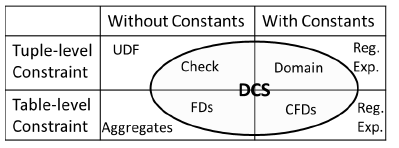
\includegraphics[scale=1]{img/quadran.png}
	\caption{A denial constraint(DC) can express many type of others constraints}
\end{figure}


\subsection{Quelques défintion et propriétés}

Dans cette sous-section, nous allons définir quelques notions et propriétés sur les DC qui ne serviront dans les chapitres qui suivront.
\subsubsection{Satisfiabilité}

\begin{mydef}
Soit $\varphi$ DC sur $S$. On dit que $\varphi$ est \emph{satisfiable} si elle peut être satisfaite par une relation non vide sur $S$, i.e Si $\exists I$ over $S$ avec $I$ non vide tel que $I \models \varphi$, alors $\varphi$ est \emph{satisfiable}.

Si $\varphi$ n'est pas satisfiable, nous dirons qu'il est \emph{insatisfiable} 
\end{mydef}

\subsubsection{Implication logique}

\begin{mydef}
Soit $\varphi_1,\varphi_2$ deux DC sur $S$. On dit que $\varphi_1$ \emph{implique} $\varphi_2$, que l'on note $\varphi_1 \models\varphi_2$, si pour chaque relation $I$ sur $S$, si $I \models \varphi_2$ alors on a $I \models \varphi_1$. On dira aussi que $\varphi_2$ est \emph{plus faible} que $\varphi_1$ ou bien que $\varphi_1$ est \emph{plus fort} que $\varphi_2$
\end{mydef}

\subsubsection{Trivial DC}

Une DC peut être inutile et toujours vraie. De telles DC ne devraint pas être présentes dans la base de données puisqu'ils ne détecteront jamais aucune violation. Dans ce cas on dira que le DC est \emph{triviale}. 
\begin{mydef}
	Une DC $\varphi$ est dite \emph{triviale} si $\forall I$ sur S, on a $I \models \varphi$
\end{mydef}

It's quite easy to discover trivial denial constraint with the following property \cite{DCs}:

\begin{myprop}
\label{trivialprop}
Soit $\varphi$ une denial constraint sur S. Alors, $\varphi$ est triviale si et seulement $\exists P_i \in pred(\varphi)$ tel que l'opérateur $\theta_i = \bot$ 
\end{myprop}



If we say for data the table \ref{tableMain}:
$$\varphi : t_\alpha,t_\beta \in R \; \neg(t_\alpha.Tax = t_\beta.Tax \wedge t_\alpha.Tax < t_\beta.Tax)$$ 

It's a trivial by property \ref{trivialprop} It's quite obvious it's impossible that two persons have the same tax rate and one's tax rate is greater than the other. For the rest of this study we won't consider trivial DCs

\subsubsection{Augmentation}

Further in this report, we'll see addition and deletion operations in order to perform data repairing on these constraints. But adding predicates to valid DCs is useless because of the augmentation property \cite{DCs}:

\begin{myprop}
	If $\varphi = \neg (P_1 \wedge P_2 \wedge ... \wedge P_n)$ is a valid DC, then $\varphi ' = \neg(P_1 \wedge P_2 \wedge ... \wedge P_n \wedge Q)$ is also a valide DC
\end{myprop}

%It's quite easy to prove this property. If $\varphi$ is valid it means every $t_\alpha \in R$ is accepted by the constraint. If it's accepted, $\forall t_\alpha$ one of the $P_i \in \varphi$ is false. So whatever $Q$ is, $t_\alpha$ will still be accepted. It's independent of the value of Q. By this way, Q is useless in $\varphi$

This property is quite trivial. Remember that $\varphi$ is a valid DC over $I$ means $I \models \varphi$ so $\forall t \in I$ we have $\neg (P_1 \wedge P_2 \wedge ... \wedge P_n)$ true. Then $\neg (P_1 \wedge P_2 \wedge ... \wedge P_n \wedge Q)$ is true too.
\subsubsection{Transitivity}
In \cite{DCs} they defined the transitivity of DCs as:

\begin{myprop}
	If $\varphi = \neg (P_1 \wedge P_2 \wedge ... \wedge P_n \wedge Q_1)$ and $\varphi ' = \neg (R_1 \wedge R_2 \wedge ... \wedge R_n \wedge Q_2)$ are both valid DCs and $Q_2 \in Imp(\overline{Q_1})$, \\ then $ \varphi '' = \neg(P_1 \wedge ... \wedge P_n \wedge R_1 \wedge ... \wedge R_n)$ is also a valid DC.
\end{myprop}

In other words if two \textbf{valid} DCs, each with one predicate that can't be false in the same time, then merging those DCs and removing the two predicates will produce a \textbf{valid} DC.

It's possible to prove that:

%\begin{proof}
%	$\forall t_\alpha \in R$, we have $\varphi$ and $\varphi '$ verified.
%	
%\hspace*{0.5cm}	We have $Q_2 \in Imp(\overline{Q_1})$ so $Q_2$ and $Q_1$ can not be true or false at the same time.
%	\begin{enumerate}
%	 \item if $Q_1$ is false, then $Q_2$ is true . Therefore $\exists R_i\ such\ as\ R_i$ is false (because $\varphi$ should be verified). $\varphi ''$ is verified too because $R_i \in \varphi ''$
%	 \item if $Q_1$ is true, then $Q_2$ is false . Therefore $\exists P_i\ such\ as\ P_i$ is false (because $\varphi$ should be verified). $\varphi ''$ is verified too because $P_i \in \varphi ''$
%	\end{enumerate}
%\end{proof}

\begin{proof}~\\
	\hspace*{0.55cm} $\varphi$ is a valid DC : $\neg (P_1 \wedge P_2 \wedge ... \wedge P_n \wedge Q_1)$ is true.
	
	$\varphi '$ is a valid DC : $\neg (R_1 \wedge R_2 \wedge ... \wedge R_n \wedge Q_2)$ is true.
	
	$Q_2 \in Imp(\overline{Q_1})$ : $Q_1 \oplus Q_2$ is true%$Q_1 \wedge Q_2$ is false 
	
	then $\neg (P_1 \wedge ... \wedge P_n) \vee \neg (R_1 \wedge ... \wedge R_n \wedge Q_2) \equiv \varphi'' $ is true \footnote{$\neg p \vee \neg Q \equiv \neg (p \wedge q)$}
\end{proof}

\subsubsection{Refinement}
\label{RefinementSection}
In \cite{main} they define the refinement of a DC as :

\begin{mydef}
% $\varphi_2$ is a \textbf{refinement} of $\varphi_1$, denoted by $\varphi_1 \preceq \varphi_2$, if for each $ P$ : $x\phi_1 y \in pred(\varphi_1)$, there exists a $Q : x \phi_2 y \in pred(\varphi_2)$ such that $\phi_1 \in Imp(\phi_2)$
 $\varphi_2$ is a \textbf{refinement} of $\varphi_1$, denoted by $\varphi_1 \preceq \varphi_2$, if for each $P_i \in pred(\varphi)$ there exists $Q_j$ such that $P_i$ is implied by $Q_j$. 
\end{mydef}

\begin{myexample}
	Let $\varphi : \neg(s.Tax \leq t.Tax \wedge s.Income > 25k)$ and $\varphi ' : \neg(s.Tax < t.Tax \wedge s.Income > 25k \wedge s.Year = t.Year)$ we have $\varphi \preceq \varphi'$ because $s.Tax \leq t.Tax$ implies $s.Tax < t.Tax$ and $s.Income > 25k$ implies $s.Income > 25k$
\end{myexample}

As we can see, if we insert an additional predicates in a DC $\varphi$ , the variant $\varphi '$ is a refinement of $\varphi$
\begin{mydef}
 $\Sigma_2$ is a \textbf{refinement} of $\Sigma_1$, denoted by $\Sigma_1 \preceq \Sigma_2$, if for each $ \varphi_2 \in \Sigma_2$, there exists a $\varphi_2 \in \Sigma_1$ such that $\varphi_1 \preceq \varphi_2$
\end{mydef}

As we can see, if you want to change less data, you should refine your DCs with insertion or substitution. For example if our DC is $t_\alpha.Tax \leq t_\beta.Tax$ and we change it to $t_\alpha.Tax < t_\beta.Tax$ you'll change less data.

\subsection{Différence par rapport à l'article de base}

\chapter{Data Repairing}

Errors are frequent in database and these anomalies can make applications unreliable. Some methods detect them but don't repair the detected anomalies. But if one simply filters the dirty data you've detected, applications could still be unreliable. \cite{anodetect} Instead of only detecting errors and filter them, it's better to repair the dirty data.\\

\begin{mydef}
We define $cell(\varphi)$ as :
$$ cell(\varphi) = \{t.A|P : t.A \phi c \in pred(\varphi) \} \cup \{t.A,s.A|P : t.A \phi s.A \in pred(\varphi) \}$$
\end{mydef}

So $cell(\varphi)$ are all the t.A involved in $\varphi$. We can also define $cell(\Sigma)$ as $\cup_{\varphi \in \Sigma} \; cell(\varphi)$ . If t.A is not in $cell(\Sigma)$, it cannot be a violation of a constraint and therefore don't need to be repair. 

The goal of data repairing is to find a modification $I'$ for an instance $I$ of $R$, in which all of the violations in the constraints set $\Sigma$ are eliminated. In other words, we want $I' \models \Sigma$ ($I'$ satisfy $\Sigma$). Data repairing process follows the minimum change principle: the data repair $I'$ have to minimize the data repair cost define as \cite{main}:
\begin{mydef}
If $I'$ is a repair for $I$ instance of $R$ by modifying attribute values without any deletion or insertion tuples, the data repair cost is:
$$ \Delta(I,I') = \sum_{t \in I, A \in attr(R)} w(t.A).dist(I(t.A),I'(t.A) $$
where :
\begin{itemize}
	\item $dist(I(t.A),I'(t.A))$ is the distance between two values on $t.A$ in $I$ and $I'$.
	\item $w(t.A)$ is the weight of cell $t.A$.
\end{itemize}
\end{mydef}

We can see that the cost can be the number of values in $cell(\varphi)$ we changed if we put:
$$
dist(I(t.A),I'(t.A)) =
\left\{
	\begin{array}{ll}
	  1 \; if I(t.A) \neq I'(t.A)\;(the\ value\ changed) \\
	  0 \; otherwhise\;(no\ changes\ were\ made)
	\end{array}
\right.
$$
We can put the distance for numerical values on the difference of the two values. For string values we can use the edit distance.\\

The weight $w(t.A)$ can show the trust of the original value in cell which is subjective or simply be a constant if we don't have a lot of knowledge about the data. For example in the table \ref{tablePerson}, we can expect a child attribute value to be more accurate than a Salary or Tax attribute value.\\

It is important to notice it is possible we are not able to find any repair $I'$ that can eliminates all the violations. Sometimes there is no value in $dom(A)$ that can fit the constraint. In that case, we use a $fresh variable$ outside the $dom(A)$ in order to extend the domain. A fresh variable is a value that does not satisfy any predicate (all predicates are false), we are sure that we can satisfy the DC. (it's satisfy if at least one of the predicates is false). Each time we are not able to find a value in the $dom(A)$  to repair a cell, we put a new fresh variable $fv$\\

Let us take an example on the table \ref{tableMain}. Let's say our Denial Constraint is the following one:

$$ \varphi : t_\alpha,t_\beta \in R, \neg(t_\alpha.Income > t_\beta.Income \wedge t_\alpha.Tax \leq t_\beta.Tax)$$

In other words, we supposed that if someone get a higher income than another person then he should paid an higher tax every year. We have $ \langle t_2,t_1 \rangle \not\models \varphi $ because $t_1$.Income < $t2.$Income and $t2$.Tax$\ \leq\ t1$.Tax. Same problem with $ \langle t_3,t_1 \rangle$, $ \langle t_5,t_1 \rangle$, ect... one can find all the violation in the figure \ref{BadTax} A repair $I'$ could be the following one:

\begin{table}[H]
	\centering
	\begin{tabular}{|c|c c c c c c c c c c|}
	\hline
	   & $t_1$ & $t_2$ & $t_3$ &$t_4$ &$t_5$ &$t_6$ &$t_7$ &$t_18$ &$t_9$ &$t_10$ \\
	\hline
	 Tax & 0 & \color{red} $fv_1$ & \color{red} $fv_2$& 3k & \color{orange}$fv_3$& \color{orange} $fv_4$& \color{orange} $fv_5$& 21k & 21k & 40k\\
	 \hline
	\end{tabular}
	\caption{\label{tableExample} Example of repair $I'$ with Tax for $\varphi$}.
\end{table}


\begin{figure}
	\centering
	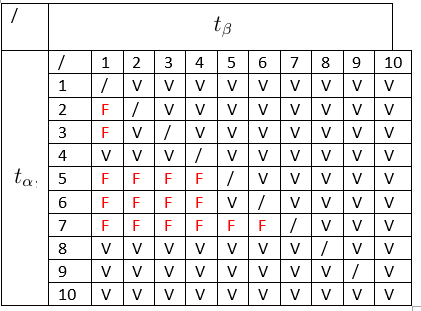
\includegraphics[scale=1]{img/TaxBad}
	\caption{\label{BadTax} All the violation for $\varphi$}
\end{figure}

The reason we put $fv_1$ as Tax value for $t_2$ is because we knew the following things:
\begin{enumerate}

\item $I(t_1.Tax)=0$ so $I'(t_2.Tax)>0$ because $I(t_1.Income)<I(t_2.Income)$
\item $I(t_3.Tax)=3$ so $I'(t_2.Tax)<3$ because $I(t_2.Income)<I(t_3.Income)$
\item $dom(Tax) = \{0,3k,21k,40k\}$

\end{enumerate}
Because we had no values in the $dom(Tax)$ that would respect 1 and 2, we need to use a fresh variable $fv_1$ out of the $dom(Tax)$. The same  logic can be used to understand why we had to use $fv_2$ to $fv_5$. We could put random value instead but it could be a problem if we insert correct value in the future (These correct values could be see as dirty one).
We only know that 0< $fv_1$,$fv_2$ <3k in order to respect 1 and 2. In the same idea, we have 3k < $fv_3$,$fv_4$,$fv_5$ < 21k.

We can compute the repair cost for $Tax$ in this table. Let's say that:\\

$$
\forall a,b \in dom(A) \ with \ a \neq b.
\left\{
	\begin{array}{ll}
	   dist(a,a)=0\\
	   dist(a,b)=1\\
	   dist(a,fv)=1.5\\
	\end{array}
\right.
$$

When we don't change anything, the distance is obviously equal to zero. $dist(a,fv)$ have to be higher than $dist(a,b)$ otherwise the cost for a non-domain value will be lower than a domain value and we want to avoid fresh variable as much as possible \footnote{it's always better to work with values in dom(A) when it's possible}. If we had $dist(a,fv)$ lower than $dist(a,b)$, any repair that uses fresh variable outside the domain would be better and of course it's not a good behavior. In our example, with the value said just before, we can compute a $\Delta(I,I')$ = 7.5

\section{Integrity constraints variations}

We saw earlier that a constraint can be overrefined failing to detect some error or in the opposite a constraint can be oversimplified leading to consider some good data as an error. Because constraints can be inaccurate we need to modify them. We'll consider two types of constraint variance: predicate deletion and in the opposite predicate insertion.\\

When we perform a predicate insertion, some tuples no longer violate the DC. With this variation we can repair a oversimplified constraint but we need to be careful otherwise the DC can be useless. We need to avoid insertion which can lead to a trivial DC or insertion of predicates with obvious constants(like $t_\alpha.Salary$<0 in the table \ref{tablePerson}). \\

An example of trivial DC is a DC $\varphi$ with a predicate $P_i$ : $x \phi_i y$ and we had another predicate $P_j$ : $x \phi_j y$ in the DC with $\overline{\phi_j} \in Imp(\phi_i)$. \\

For overrefined DCs, we need to remove some predicates but we need to be careful. If too many predicates are withdraw, we can get an new oversimplified DCs. The more the predicates are deleted, the higher the data repair cost will be as stated in the Lemma1 in \cite{main}. In the other hand the more the predicates are added, the lower the data repair will be. So if you add more predicates than you remove, there will be less data to change. In the opposite, if you remove more predicates than you add, there will be more data to change. The \emph{data repair cost function} take this effect into consideration. It count positively predicate insertion and negatively predicate addition. For $\Sigma '$ a variant of $\Sigma$ in which all $\varphi ' \in \Sigma '$ are obtained by insertion or deletion of predicates for corresponding $\varphi \in \Sigma$, in \cite{main} they define the constraint variation cost:

\begin{mydef}
For a variant $\Sigma '$ of $\Sigma$, the contraint variation cost is defined as

$$\Theta (\Sigma,\Sigma ') = \sum_{\varphi in \Sigma} edit(\varphi,\varphi ')$$

\hspace*{2cm} where $\varphi '$ is a variant of $\varphi$ and $edit(\varphi,\varphi ')$ is the corresponding cost.
\end{mydef}

the $edit(\varphi , \varphi ')$ indicates the cost of changing $\varphi$ to $\varphi'$ is defined as:
\begin{mydef}
$$
 edit(\varphi, \varphi') = \sum_{P \in \varphi \setminus \varphi'} c(P) + \lambda \sum_{P \in \varphi' \setminus \varphi} c(P)$$
 
where $c(P)$ denote the weighted cost of predicate P and $\lambda$ is the weight of a deletion compare to an addition and -1<$\lambda$<0.
\end{mydef}

We don't have to use $\lambda$ =-1 otherwise a deletion followed by an addition would have a cost equal to 0(and it's a bad idea for predicate substitution). For example if we have:

$$ \varphi : t_\alpha,t_\beta \in R, \neg(t_\alpha.Income > t_\beta.Income \wedge t_\alpha.Tax \leq t_\beta.Tax)$$

This DC express the fact that if I get a higher income than someone else, i should pay a higher tax rate. We'll change this DC by deleting $t_\alpha.Tax \leq t_\beta.Tax$ and add $t_\alpha.Tax < t_\beta.Tax$. It can express the fact that someone with a very low Income could get a Tax equals to 0.

$$ \varphi ' : t_\alpha,t_\beta \in R, \neg(t_\alpha.Income > t_\beta.Income \wedge t_\alpha.Tax < t_\beta.Tax)$$

The constraint variation with $\lambda$ = $\frac{1}{2}$ and $c(P)$ = 0 is : $edit(\varphi, \varphi') = c(t_\alpha.Tax < t_\beta.Tax) + \frac{1}{2} c(\alpha.Tax \leq t_\beta.Tax)$ = $\frac{1}{2}$. \\

With this new constraint, we got less violations. All the violations can be found the figure \ref{GoodTax}. The modifications we made in table \ref{tableExample} are:

\begin{table}[H]
	\centering
	\begin{tabular}{|c|c c c c c c c c c c|}
	\hline
	   & $t_1$ & $t_2$ & $t_3$ &$t_4$ &$t_5$ &$t_6$ &$t_7$ &$t_18$ &$t_9$ &$t_10$ \\
	\hline
	 Tax & 0 & 0 & 0 & \textcolor{red}{0} & 0 & 0 & 0 & 21k & 21k & 40k\\
	 \hline
	\end{tabular}
	\caption{\label{tableExample2} Example of repair with Tax}.
\end{table}


\begin{figure}
	\centering
	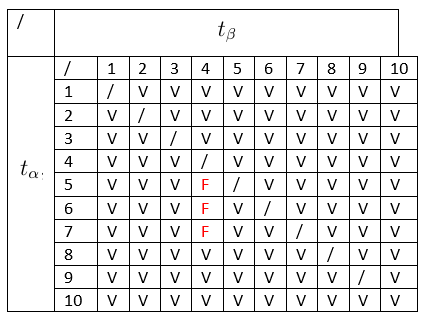
\includegraphics[scale=1]{img/TaxGood}
	\caption{\label{GoodTax} All the violation for $\varphi '$}
\end{figure}

Indeed, a repair for a column with one correction is better than the previous repair with 5 fresh variables (see table \ref{tableExample}) as a correction. On our new DC, only the ($t_4.Tax$)=3k have to be changed with the value 0. Further in this thesis, we'll see how we can reach these repairs.

When we do constraint modification, we should not consider the case where we delete an entire constraint.  We should not remove all the predicates because a DC like $\neg()$ doesn't mean anything. We can't even say if it's always true or always false.

\subsection{Maximal Constraint Variants}

	Every constraint variant $\Sigma'$ with cost $\Theta(\Sigma,\Sigma')$ shouldn't be considered. They're some variation that we're sure they are worst than any another? To perform a prunning of constraints variant that doesn't generate minimum data repair, we'll use the definition of refinement we explained in the previous chapter at the section \ref{RefinementSection}.
	
\begin{mydef}\cite{main}
 We say that a variant $\varphi '$ of a constraint $\varphi$ with $\varphi \preceq \varphi'$ is \textbf{maximal}, if there does not exist another $\varphi ''$ such that $\varphi ' \preceq \varphi ''$ and $edit(\varphi,\varphi'') = edit (\varphi,\varphi')$
\end{mydef}

\begin{myprop}\cite{main}

For any inserted predicate $ P $ : $x \phi y \in pred(\varphi ') \setminus pred(\varphi)$, if $\phi \in \{\leq,\geq,\neq \}$, then $\varphi '$ is not maximal.

\end{myprop}

This property comes from the $Imp(\varphi)$ definition. If $Varphi_1 \in Imp(\varphi_2)$ then $a\varphi_1 b$ implies $a \varphi_2 b$. $\leq \geq$ and $\neq$ are the 3 operators who implies operator that are no themselves (see table \ref{tableImp}). With this property we see that it's useless to insert every predicate that you're able to construct. We only have to insert predicates with operators {>,<,=} when considering variants of $\varphi$ Let's illustrate that with an example. We'll take two denial constraint on table \ref{tableMain} for this.
$$\varphi_1 : \forall t_\alpha,t_\beta \in R, \neg( t_\alpha.Name = t_\beta.Name \wedge t_\alpha.Income = t_\beta.Income \wedge t_\alpha.CP \neq t_\beta.CP )$$
$$\varphi_2 : \forall t_\alpha,t_\beta \in R, \neg( t_\alpha.Name = t_\beta.Name \wedge t_\alpha.Income \leq t_\beta.Income \wedge t_\alpha.CP \neq t_\beta.CP )$$


We know that $\leq \in Imp(=)$ (see table \ref{tableImp}) for Income so we have $\varphi_2 \preceq \varphi_1$. By the last property we know that $\varphi_2$ is not maximal because it contains $\leq$ operator. In this scenario the data repair cost is 7 for $\varphi_2$ and $\varphi$ will get a data repair cost equal to 3. 

\begin{table}[H]
	\parbox{.45\linewidth}{
	\centering
	\begin{tabular}{|c|c c c|}
	\hline
	    & Name & Cellphone Number & Income\\
	\hline
	 t1 & Ayres & \color{red}564-389 & \color{red}22k\\
	 t2 & Ayres & \color{red}564-389 & 22k\\
	 t3 & Ayres & 564-389 & 22k\\
	 t4 & Stanley &\color{red} 930-198 &\color{red}24k\\
	 t5 & Stanley &\color{red} 930-198 & 24k\\
	 t6 & Stanley & 930-198 & 24k\\
	 t7 & Dustin & \color{red}824-870 & \color{red}100k\\
	 t8 & Dustin & \color{red}824-870 & 100k\\
	 t9 & Dustin & 824-870 & 100k\\
	 t10 & Dustin & \color{red}824-870 & \color{red}100k\\
	 \hline
	\end{tabular}
	\caption{Correction with $\varphi_2$: 7 changes needed only for the collumn CP.}.
	}
	\hfill
	\parbox{.45\linewidth}{
	\centering
	\begin{tabular}{|c|c c c|}
	\hline
	    & Name & Cellphone Number & Income\\
	\hline
	 t1 & Ayres & 322-573 & 21k\\
	 t2 & Ayres & \color{red} 564-389 & 22k\\
	 t3 & Ayres & 564-389 & 22k\\
	 t4 & Stanley & 868-701 &23k\\
	 t5 & Stanley & \color{red} 930-198 & 24k\\
	 t6 & Stanley & 930-198 & 24k\\
	 t7 & Dustin & 179-924 & 25k\\
	 t8 & Dustin & \color{red} 824-870 & 100k\\
	 t9 & Dustin & 824-870 & 100k\\
	 t10 & Dustin & 387-215 & 150k\\
	 \hline
	\end{tabular}
	\caption{Correction with $\varphi_1$ : only 3 changes are needed.}.
	}
\end{table}



We see that the refinement got a better data repair cost. It's not a coincidence because the following lemma exist: \cite{main}

\begin{mylemma}
 Given two constraints variants $\Sigma_1,\Sigma_2$ of $\Sigma$ such that $\Sigma_2$
 is also a refinement of $\Sigma_1$, have $\Sigma \preceq \Sigma_1 \preceq \Sigma_2$, is always has $\Delta(I,I_1) \geq \Delta(I,I_2)$, where $I_1$ and $I_2$ are the minimum data repairs with regards to $\Sigma_1$ and $\Sigma_2$, respectively.
\end{mylemma}

As a consequence of this Lemma, any non-maximal set of denial constraint $\Sigma$ can be removed from the possibilities of good repair

\subsection{Pruning our candidates}

In this subsection we'll focus on removing the constraint variant $\Sigma '$ that can't generate the minimum data repair. We already have seen that $\Sigma$ with a non maximal constraint $\varphi$ can be remove. To go further, we will  consider two bounds of possible minimum data repairs cost for the instance $I$ : the lower bound noted as $\delta_l(\Sigma',I)$ and the upper bound noted $\delta_u(\Sigma,I)$. We consider the following property:

\begin{myprop}
\label{boundRemove}
	For two constraints variants $\Sigma_1$ and $\Sigma_2$ for the instance $I$ of $R$, if $\delta_u(\Sigma_1,I) < \delta_l(\Sigma_2,I)$ then $\Sigma_2$ can be discarded.
\end{myprop}

It means the worst bound(upper) of repair for $\Sigma_1$ is still better than the best bound(lower) of repair for $\Sigma_2$, then $\Sigma_2$ is useless and can be ignored.

\subsubsection{Conflict Graph}

Now, we'll introduce the conflict graph which can represent the violations in an instance $I$ of $R$. In the first place, we need to find all the violations and we could get the data repair cost bound from them. We define the violation set as: \cite{main}

\begin{mydef}
 The violation set noted as $viol(I,\varphi) = \{ \langle t_i,t_j,... \rangle | \langle t_i,t_j,... \rangle \not\models \varphi $ with $ t_i,t_j,... \in I \}$ is a set of tuple lists that violate $\varphi$. The violation set of $\Sigma$ is $viol(I,\Sigma) = \cup_{\varphi \in \Sigma}viol(I,\varphi)$.
\end{mydef}

\begin{figure}
 \centering
\hspace*{-1.8cm} 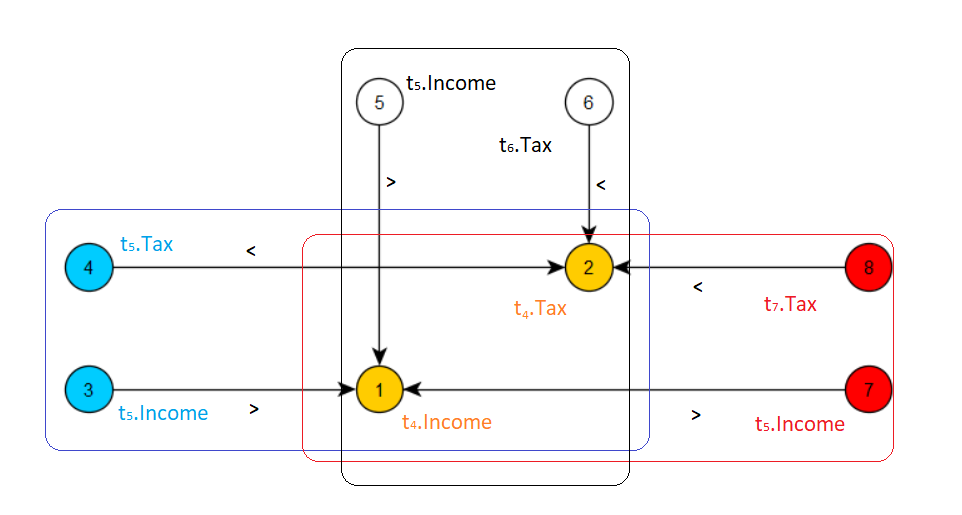
\includegraphics[scale=1]{img/grapht4.png}
 \caption{\label{grapht4} Conflict hypergraph for $\varphi$}
\end{figure}

With the conflict hypergraph $G$ we can represent the violations in I. For each violation tuples $ \langle t_i,t_j,...\rangle \in viol(I,\varphi)$ there are an edge for $cell(t_i,t_j,...,\varphi)$ in G. A good repairing $I'$ consists in correcting the data base to be able to remove all the edges on the graph. The hypergraph of $I'$ should be empty.

Let's take an example on the table \ref{tableMain} with a denial constraint we already used:

$$\varphi': \forall t_\alpha,t_\beta \in R , \neg(t_\alpha.Income > t_\beta.Income \wedge t_\alpha.Tax < t_\beta.Tax)$$

For this relation the violation set is (see Figure \ref{GoodTax}):
 $$ viol(I,\varphi') = \{ \langle t_5,t_4 \rangle,\langle t_6,t_4 \rangle,\langle t_7,t_4 \rangle \}$$

On our hypergraph, $\langle t_5,t_4 \rangle \in viol(I,\varphi')$ consist of $cell(t_5,t_4;\varphi')$ which is equal to $\{ t_5.income,t_4.Income,t_5.Tax,t_4.Tax\}$. We want to remove a vertex, i.e eliminate a conflict. Let's first introduce some definition and a Lemma: \cite{main}

\begin{mydef}
	We denote $ \min_{a \in dom(A)} dist(I(t.A),a) $ the weight of a vertex t.A, i.e, the minimum cost should be paid to repair t.A.
\end{mydef}

\begin{mydef}
	$\mathbb{V}(G)$ is the \textbf{minimum weighted vertex cover} of the hypergraph G corresponding to $\Sigma$ with weight
	$$||\mathbb{V*(G)}|| = \sum_{t.A \in \mathbb{V}(G)} min_{a\in dom(A)} dist(I(t.A),a)$$
\end{mydef}

\begin{mylemma}
	For any valid repair $I'$ of $I$, i.e, $I' \models \Sigma$, we have $\Delta(I,I') \leq ||V*(G)||$. 
\end{mylemma}

%Computing $\mathbb{V}$ is a NP-Hard problem so we need to approximate it. We'll consider an constant factor-f approximation of $\mathbb{V}$ which is $\frac{||\mathbb{V}(G)||}{||\mathbb{V}*(G)||} \leq f$. where f is the maximum degree of hyperedges and $||\mathbb{V}(G)||$ is an approximation of $||\mathbb{V}*(G)||$.

In \cite{main} they define the upper and lower bound of repair cost in this way :
$$ \delta_l(\Sigma,I) = \frac{||\mathbb{V}(G)||}{Deg((\Sigma)}$$
$$ \delta_u(\Sigma,I) = \sum_{t.A \in \mathbb{V}(G)} dist(I(t.A),fv)$$

If we come back to our example and suppose that we have :
$$
\forall a,b \in dom(A) \ with \ a \neq b.
\left\{
	\begin{array}{ll}
	   dist(a,a)=0\\
	   dist(a,b)=1\\
	   dist(a,fv)=1.1\\
	\end{array}
\right.
$$

So if each vertex has a weight of 1 (=$ dist(a,b)$) and if we put $\mathbb{V}(G)$ = $\{t_4.Tax \}$ we get $||\mathbb{V}(G)||$ = 1. We also have $Deg(\varpi')$ = 4, so with formula we have we know upper and lower bound : $\delta_l(\Sigma,I)$=$\frac{||\mathbb{V}(G)||}{Deg((\Sigma)}$ = $\frac{1}{4}$ = 0.25 and $\delta_u(\Sigma,I) = \sum_{t.A \in \mathbb{V}(G)} dist(I(t.A),fv)$ = $dist(a,fv)$=1.1 .


\section{$\theta$-tolerant model}

In this section we'll talk about the $\theta$-tolerant repair model which is the main models we want to study. $\theta$ is a threshold on the variation on the set of constraint $\Sigma$, so we don't want a constraint variation cost greater than $\theta$ : $\Theta(\Sigma,\Sigma') \leq \theta$. It helps to avoid any kind of over-refinement and so some undetected dirty data. To avoid the over-simplification and identify correct data as dirty data, the repairing should pursue the minimum change principle. We need to find a repair $I'$ of the original instance $I$ and minimize the repair cost $\Delta(I,I')$.\\

Finding the best (minimum) $\theta$-tolerant repair is difficult, it's a NP-hard problem. An NP-hard problem is a class of decision problems which are at least as hard as the hardest problems in NP \footnote{problems whose a solution can be verified as good one in a polynomial time}. What we have to remind is it's not possible to resolve it in a polynomial time. Even is the first approach we could made is to get all the constraints variant $\Sigma'$ and then compute $\Theta(\Sigma,\Sigma')$, look if it's lower than $\theta$ and then find the minimum data repair $I'$. But this way is oviously high in complexity\\

We saw that we could replace some value by a fresh variable $fv$. It's better to not turn all of them in a fresh variable mainly because $fv$ is not $dom(A)$ and also a repair like this will never return the optimal repair because we want to minimize the repair cost. \\

Now, consider $\mathbb{D}$ = $\Sigma_1 ' x \Sigma_2' x ... \Sigma_{|\Sigma|}'$ where each $\Sigma_i' \in \mathbb{D}$ is a variant of $\Sigma$ obtained by previous variations. Consider those variations bounded by $\theta$ so we have $\Theta(\Sigma,\Sigma') \leq \theta$. The algorithm \ref{tetha} return the best instance $I_{min}$ for our set of constraint variation $\Sigma$. The algorithm is simple. For each $\Sigma_i$ , if the lower bound is lower than the previous upper bound (remember the property \ref{boundRemove}). we update the value of $\delta_{min}$ if a better repaired instance comes from $I_i$. \\

\IncMargin{1em}
\begin{algorithm}
\label{tetha}

	\DontPrintSemicolon
  \caption{$\theta$-TolerantRepair$(\mathbb{D},\Sigma,I)$}
  \LinesNumbered
    \SetKwInOut{Input}{Input}
    \SetKwInOut{Output}{Output}

   % \underline{$\theta$-TolerantRepair} $(\mathbb{D},\Sigma,I)$\;
    \Input{Instance $I$, a constraint set $\Sigma$, a set $\mathbb{D}$of constraint variants with variation bound by $\theta$ }
    \Output{A minimum data repair $I_{min}$}
    $\delta_{min}$ = $\delta_u(\Sigma,I)$\;

	\For{each constraint variant $\Sigma_i \in \mathbb{D}$}{
    	\If{$\delta_l (\Sigma_i,I) \leq \delta_{min}$}
    		{
    		$I_i$ = DATAREPAIR($\Sigma_i,I,\mathbb{V}(G_i),\delta_{min}$\;
    		\If{$\Delta(I,I_i) \leq \delta_min$}
    		{$\delta_{min}$ = $\Delta(I,I_i)$\;
    		$I_{min}$ = $I_i$\;}
    		}   		
    		
	}
	\Return $I_{min}$

\end{algorithm}\DecMargin{1em}


To get an example , imagine we have for a $\theta$ = $\frac{1}{2}$ , a set of constraint variation $\mathbb{D}$ = $\{\Sigma_1,\Sigma_2\}$ with the first set of constraints $\Sigma_1$ = $\{\varphi'\}$ and the second set of constraints $\Sigma_2$ = $\{\varphi''\}$ with:
$$\varphi': \forall t_\alpha,t_\beta \in R , \neg(t_\alpha.Income > t_\beta.Income \wedge t_\alpha.Tax < t_\beta.Tax)$$
$$\varphi'': \forall t_\alpha,t_\beta \in R , \neg(t_\alpha.Income > t_\beta.Income \wedge t_\alpha.Tax = t_\beta.Tax)$$

We already have done the conflict hypergraph for $\varphi$ in figure \ref{grapht4} we also know that $\delta(\Sigma_1,I)=1.1$\\

For $\Sigma2$ we obtain the hypergraph in figure \ref{graphSigma2} (and the violations in figure \ref{EqualTax}) with $\mathbb{V}(G_2)$ = $\{ t_2.Tax,t_3.Tax,t_5.Tax,t_6.Tax,t_7.Tax\}$. We have $Deg(\Sigma_2)$ = $Deg(\varphi')$ \footnote{same reasoning: 4 cells involved.}, so we have $\delta_l(\Sigma_2,I)$= $\frac{6}{2}$ = 1,5. Remember that $\delta_u(\Sigma_1,I)$ =1.1, so we have $\delta_u(\Sigma_1,I) < \delta_l(\Sigma_2,I)$ which means we can ignore $\Sigma2$ and don't call the DATAREPAIR function on it. We will talk about the DATAREPAIR function later.

\begin{figure}
\centering
\hspace*{-1.8cm} 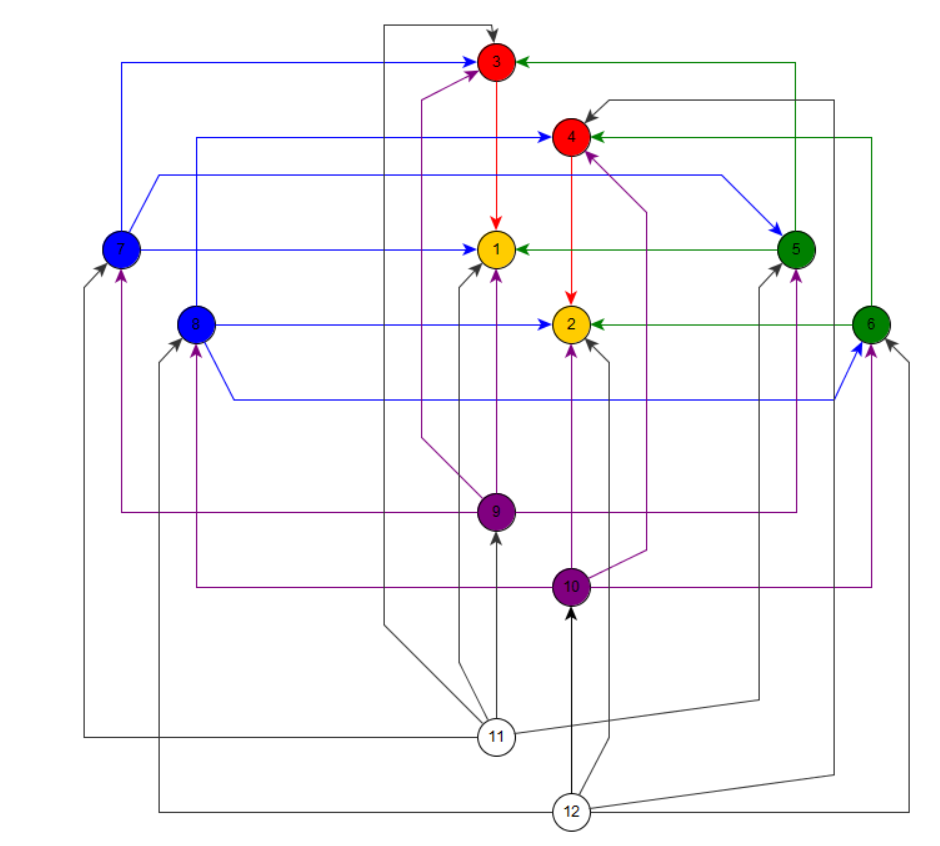
\includegraphics[scale=0.95]{img/graph2}
\caption{\label{graphSigma2}Conflict hypergraph for $\Sigma_2$ with :}
	odd number for Tax, even number for Income. \\
	$t_1$ in yellow, $t_2$ in red, $t_3$ in green,\\
	$t_4$ in blue, $t_5$ in purple and $t_6$ in white.
\end{figure}

\begin{figure}
\centering
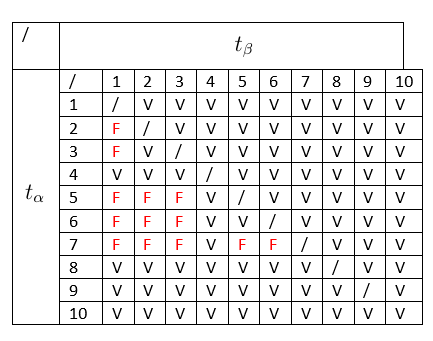
\includegraphics[scale=1]{img/TaxEqual}
\caption{\label{EqualTax}All the violations for $\varphi''$}
\end{figure}

Let's talk about the complexity. If we say that $l$ is the maximum number involved in a constraint of $\Sigma$ then we can say that the construction of $G_i$ for each $\Sigma_i \in \mathbb{D}$ cost $O(|I|^l)$. The data repairing algorithm get a complexity in time of $O(|I|^l)$ and the algorithm \ref{tetha} runs in $O(|I|^l|\mathbb{D}|)$ time. Usualy a denial constraint get 2 tuples \cite{main}.

\section{Minimum Data Repair and Violation Free}

After using the $\theta$-tolerant model, we know which constraint set $\Sigma'$ derived from $\Sigma$ we have to use to perform a repairing. But we haven't see how to repair yet. In this section we'll focus on the minimum data repair $I'$ based on the $\Sigma'$. To make this we'll use the violation free principle to be sure we don't create any violation after correcting one data. For example, if we put $t5.Tax$ to 22, we solved the violation $ \langle t_5,t_4 \rangle$ we had with $\varphi'$ \footnote{remember the $\varphi: \forall t_\alpha,t_\beta \in R , \neg(t_\alpha.Income > t_\beta.Income \wedge t_\alpha.Tax < t_\beta.Tax)$ we used many times}but we introduce a new violation $\langle t_8,t_5 \rangle$.\\

Remember we already said that finding a minimum repairing is NP-hard problem. For this reason we need to make some approximation in order to repair. For the following explanation and definition we'll note $\mathbb{C}$ the selected cells $\mathbb{V}(G)$

\subsection{Suspect identification}

\begin{mydef} \cite{main}
	The suspect set $susp(\mathbb{C},\varphi)$ of a $\varphi$ is a set of tuple lists $\langle t_i,t_j,...:\varphi \rangle$ satisfying all the predicates in $\varphi$ which do not involve cells in $\mathbb{C}$.
\end{mydef}

and they satisfy the suspect condition:

\begin{displaymath}
\begin{split}
sc(t_\alpha,t_\beta,...:\varphi) &= \{I(v_1)\phi c| P: v_1 \phi c \in pred(\varphi),v_1 \in \mathbb\{C\}\}\cup \\
	&\{I(v_1)\phi v_2| P: v_1 \phi v_2 \in pred(\varphi),v_1,v_2 \in \mathbb\{C\}\}
\end{split}
\end{displaymath}

Any violation is of course in the suspect list, which lead to the trivial lemma:

\begin{mylemma}
	For any $\mathbb{C}$, it always has $viol(I,\varphi) \subseteq susp(\mathbb{C},\varphi)$
\end{mylemma}

And by this way, if we catch all the suspect, we also get all the violation.\\

To explain it, let's return on the example $\varphi'$ related with the hypergraph at figure \ref{grapht4}. We will change only $t_4.Tax$ as we made in the table \ref{tableExample}. So we have $\mathbb{C}$ =  $\{ t_4.Tax \}$ and $susp(\mathbb{C},\varphi') = \{\langle t_4 , t_1\rangle , 
\langle t_4 , t_2\rangle,
\langle t_4 , t_3\rangle,
\langle t_5 , t_4\rangle,
\langle t_6 , t_4\rangle,
\langle t_7 , t_4\rangle,
\langle t_8 , t_4\rangle,
\langle t_9 , t_4\rangle,
\langle t_{10} , t_4\rangle \}$ If we get $\langle t_4 , t_1\rangle$ ,   we have $t_4.Income > t_1.Income$ but there is a chance that any change on $t_4.Tax$ leads to a new violation($I'(t_4.Tax)<I(t_1.Tax) $. This is the reason why it's on the suspect list. In the figure \ref{fig3} we have a graph in which every cells not in $\mathbb{C}$ are represented by circles and cell in $\mathbb{C}$ are represented by squares. Red arrows are respected predicates and blue arrows are respected predicates.


\begin{figure}
	\centering
	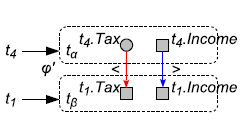
\includegraphics[scale=1]{img/fig3}
	\caption{\label{fig3}Suspect condition} 
	represented by blue arrows and repair \\
	context represented by red arrows \\
	 (with inverse operator).
\end{figure}

\subsection{Repair context over suspects}

We can now define a repair context. The repair contest of a suspect tuple is something that makes sure the suspects will not satisfy the predicates declared on $\mathbb{C}$. The reason why we need it is because a denial constraint needs at least one false predicate for every rows of the database. The repair context takes the inverse operator of predicates in $\mathbb{C}$. In \cite{main}, the repair context $rc(t_i,t_j,...:\varphi)$ of a suspect $\langle t_i,t_j,... \rangle $is defined as:

\begin{mydef}
	\begin{displaymath}
	\begin{split}
	rc(t_\alpha,t_\beta,...:\varphi) =
	&\{ I'(v_1)\overline{\phi}c|P : v_i\phi c \in pred(\varphi),v_1 \in \mathbb{C}\}\cup\\
	&\{I'(v_1)\overline{\phi} I'(v_2)|P : v_i\phi v_2 \in pred(\varphi),v_1,v_2 \in \mathbb{C}\}\cup\\
	&\{I'(v_1)\overline{\phi} '(v_2)|P : v_i\phi v_2 \in pred(\varphi),v_1,\in \mathbb{C},v2 \not\in \mathbb{C}\}\cup\\
	&\{I(v_1)\overline{\phi} I'(v_2)|P : v_i\phi v_2 \in pred(\varphi),v_2 \in \mathbb{C},v_1 \not\in \mathbb{C}\}.
	\end{split}
	\end{displaymath}
\end{mydef}

\begin{myprop}
Any assignment that satisfies all the repair contexts forms a valid repair $I'$ without introducing any new violations, i.e, $I' \preceq \Sigma$
\end{myprop}

If we continue with our previous example with $\varphi'$, we have $rc(t_4,t_1:\varphi')$ = $\{I'(t_4.Tax \geq I(t_1.Tax)\}$ , $\geq$ is the inverse operator of $<$ and we only consider predicates of $\varphi'$ with cells from $\mathbb{C}$ which are red arrows on the figure \ref{fig3}. We also have $rc(t_5,t_4:\varphi')$ = $\{I'(t_5.Tax \geq I(t_4.Tax)\}$. With both of these repair constraint we have $0 = t_1.Tax \leq t_4.Tax \leq t_5.Tax =0$ which lead to only one possible value : $t_4.Tax =0$. Remember that previously we put a fresh variable $fv$ instead of 0 (see the table \ref{tableExample} in the previous chapter).\\

We want a repair cost as small as possible, which leads to to minimize the repair cost under repair cost constraint. We have to solve the following problem:
\begin{displaymath}
\begin{split}
& \hspace*{1cm} \min \sum_{t_i.A \in \mathbb{C}} dst(I(t_i.A),I'(t_i.A)) \\
 &\ under\ the\ constraint : rc(t_i,t_j,...:\varphi)\ with\ \langle t_i,t_j,... \rangle \in susp(\mathbb{C},\varphi),\varphi \in \Sigma
\end{split}
\end{displaymath}

But it could be possible we can't assign any value (in our domain) that can fit all the repair context. In these case, we can't put any value except a fresh variable. If we decide to assign a fresh variable $fv$ to a cell can remove every repair context with this cell. The reason is that $fv$ are defined as a way they don't satisfy any kind of predicates which include predicates in repair context. If we are not able to solve our problems i.e we can't found value in dom(A) for a repaired instance $I'$, we'll assign a fresh variable until the problems is solvable. It's better to start by cells with the largest number of appearance in predicates in the repair context. We can say $I'(t.A)$ = $fv$ if $rc(t.A,\Sigma)$ which represent all the repair context declared between a constant or between $t.A$ and $v_i \not\in \mathbb{C}$.\\

If we come back to one of our first example : $\varphi : t_\alpha,t_\beta \in R, \neg(t_\alpha.Income > t_\beta.Income \wedge t_\alpha.Tax \leq t_\beta.Tax)$  For $t_2$ we have $rc(t_2.Tax,\{ \varphi \}) = \{ I'(t_2.Tax) > I(t_1.Tax),I(t_4.Tax) > I'(t_2.Tax),I(t_8.Tax) > I'(t_2.Tax),I(t_9.Tax) > I'(t_2.Tax),I(t_{10}.Tax) > I'(t_2.Tax) \}$ In the same way we did for $\varphi'$, here we have $0 = I(t_1.Tax)< I'(t_2.Tax) < I(t_4.Tax) = 3k$ and there is no value who respect it in dom(A) = $\{ 0,3k,21k,40 \}$. The only possible solution in this case is to assign a fresh variable $fv$ to $t2.Tax$. When we do this, we can remove every red arrows related from the hypergraph. But we didn't solve all of the repair contexts.
\section{Other repairing}
TODO
\subsection{Holistic data repair}
\subsection{...}

\chapter{Implementation and comparison with others models}
TODO
\chapter{Conclusion}
TODO

\bibliographystyle{plain}


\bibliography{biblio}

\newpage
\appendix
\end{document}